The Pozyx Creator Kit comes with anchors and several tags. Anchors are mounted 
on the walls and are used to position the tags. Multiple tags may be positioned
at the same time.
The Pozyx Creator kit uses ultrawideband (UWB) signals with the two-way ranging protocol to localize the tag. 
The tag is mounted on custom 3D printed wearables which the participant can wear as 
a wrist-watch or a necklace. Through trial-and-error and consultation with the Pozyx Creator Documentation
\cite{noauthor_hardware_nodate,noauthor_configuration_nodate}
it was determined that the accuracy of the system depends on factors listed below:

\begin{itemize}
    \item Number of anchors
    \item Position of anchors
\end{itemize}

These variables were modified to achieve satisfactory actual position error
and standard deviation below the expected error of 30 cm for UWB systems. The 
protocol for obtaining data and evaluating the actual position error and 
standard deviation will be described.

% ----------------------------------------------------------------------------------------------------
\section{Methodology}
This protocol tests the X, Y, and Z positional accuracy of the Pozyx Creator system in the Independent
Living Suite (ILS) at the Glenrose Rehabilitation Hospital by having a participant stand at 
a specific location in each room. Permanent appliances or furniture such as the stove
or dining table were used as much as possible to ensure that the experiment is repeatable.

\subsection{Setup}
Masking tape was used to mark the locations where the participant should place their feet.
The following procedure was followed to place the tape:
\begin{enumerate}
    \item Using a measuring tape, measure 1 meter out from the middle of the 
    appliance or furniture and place a 20 cm piece of tape centered on, perpendicular to
    and underneath the measuring tape (the tips of the participant's toes should be 1 meter
    away from the appliance).\label{step 1}
    \item Place parallel tape on the sides of the tape placed in Step \ref{step 1} to constrain
    the feet to a box. (The participant should have their toes on the tape perpendicular to the
    measuring tape and usually facing the appliance or furniture).
    Figure \ref{fig:tape} outlines some examples of tape placements.
\end{enumerate}


\begin{figure}[ht]
    \label{fig:tape}
    \centering
    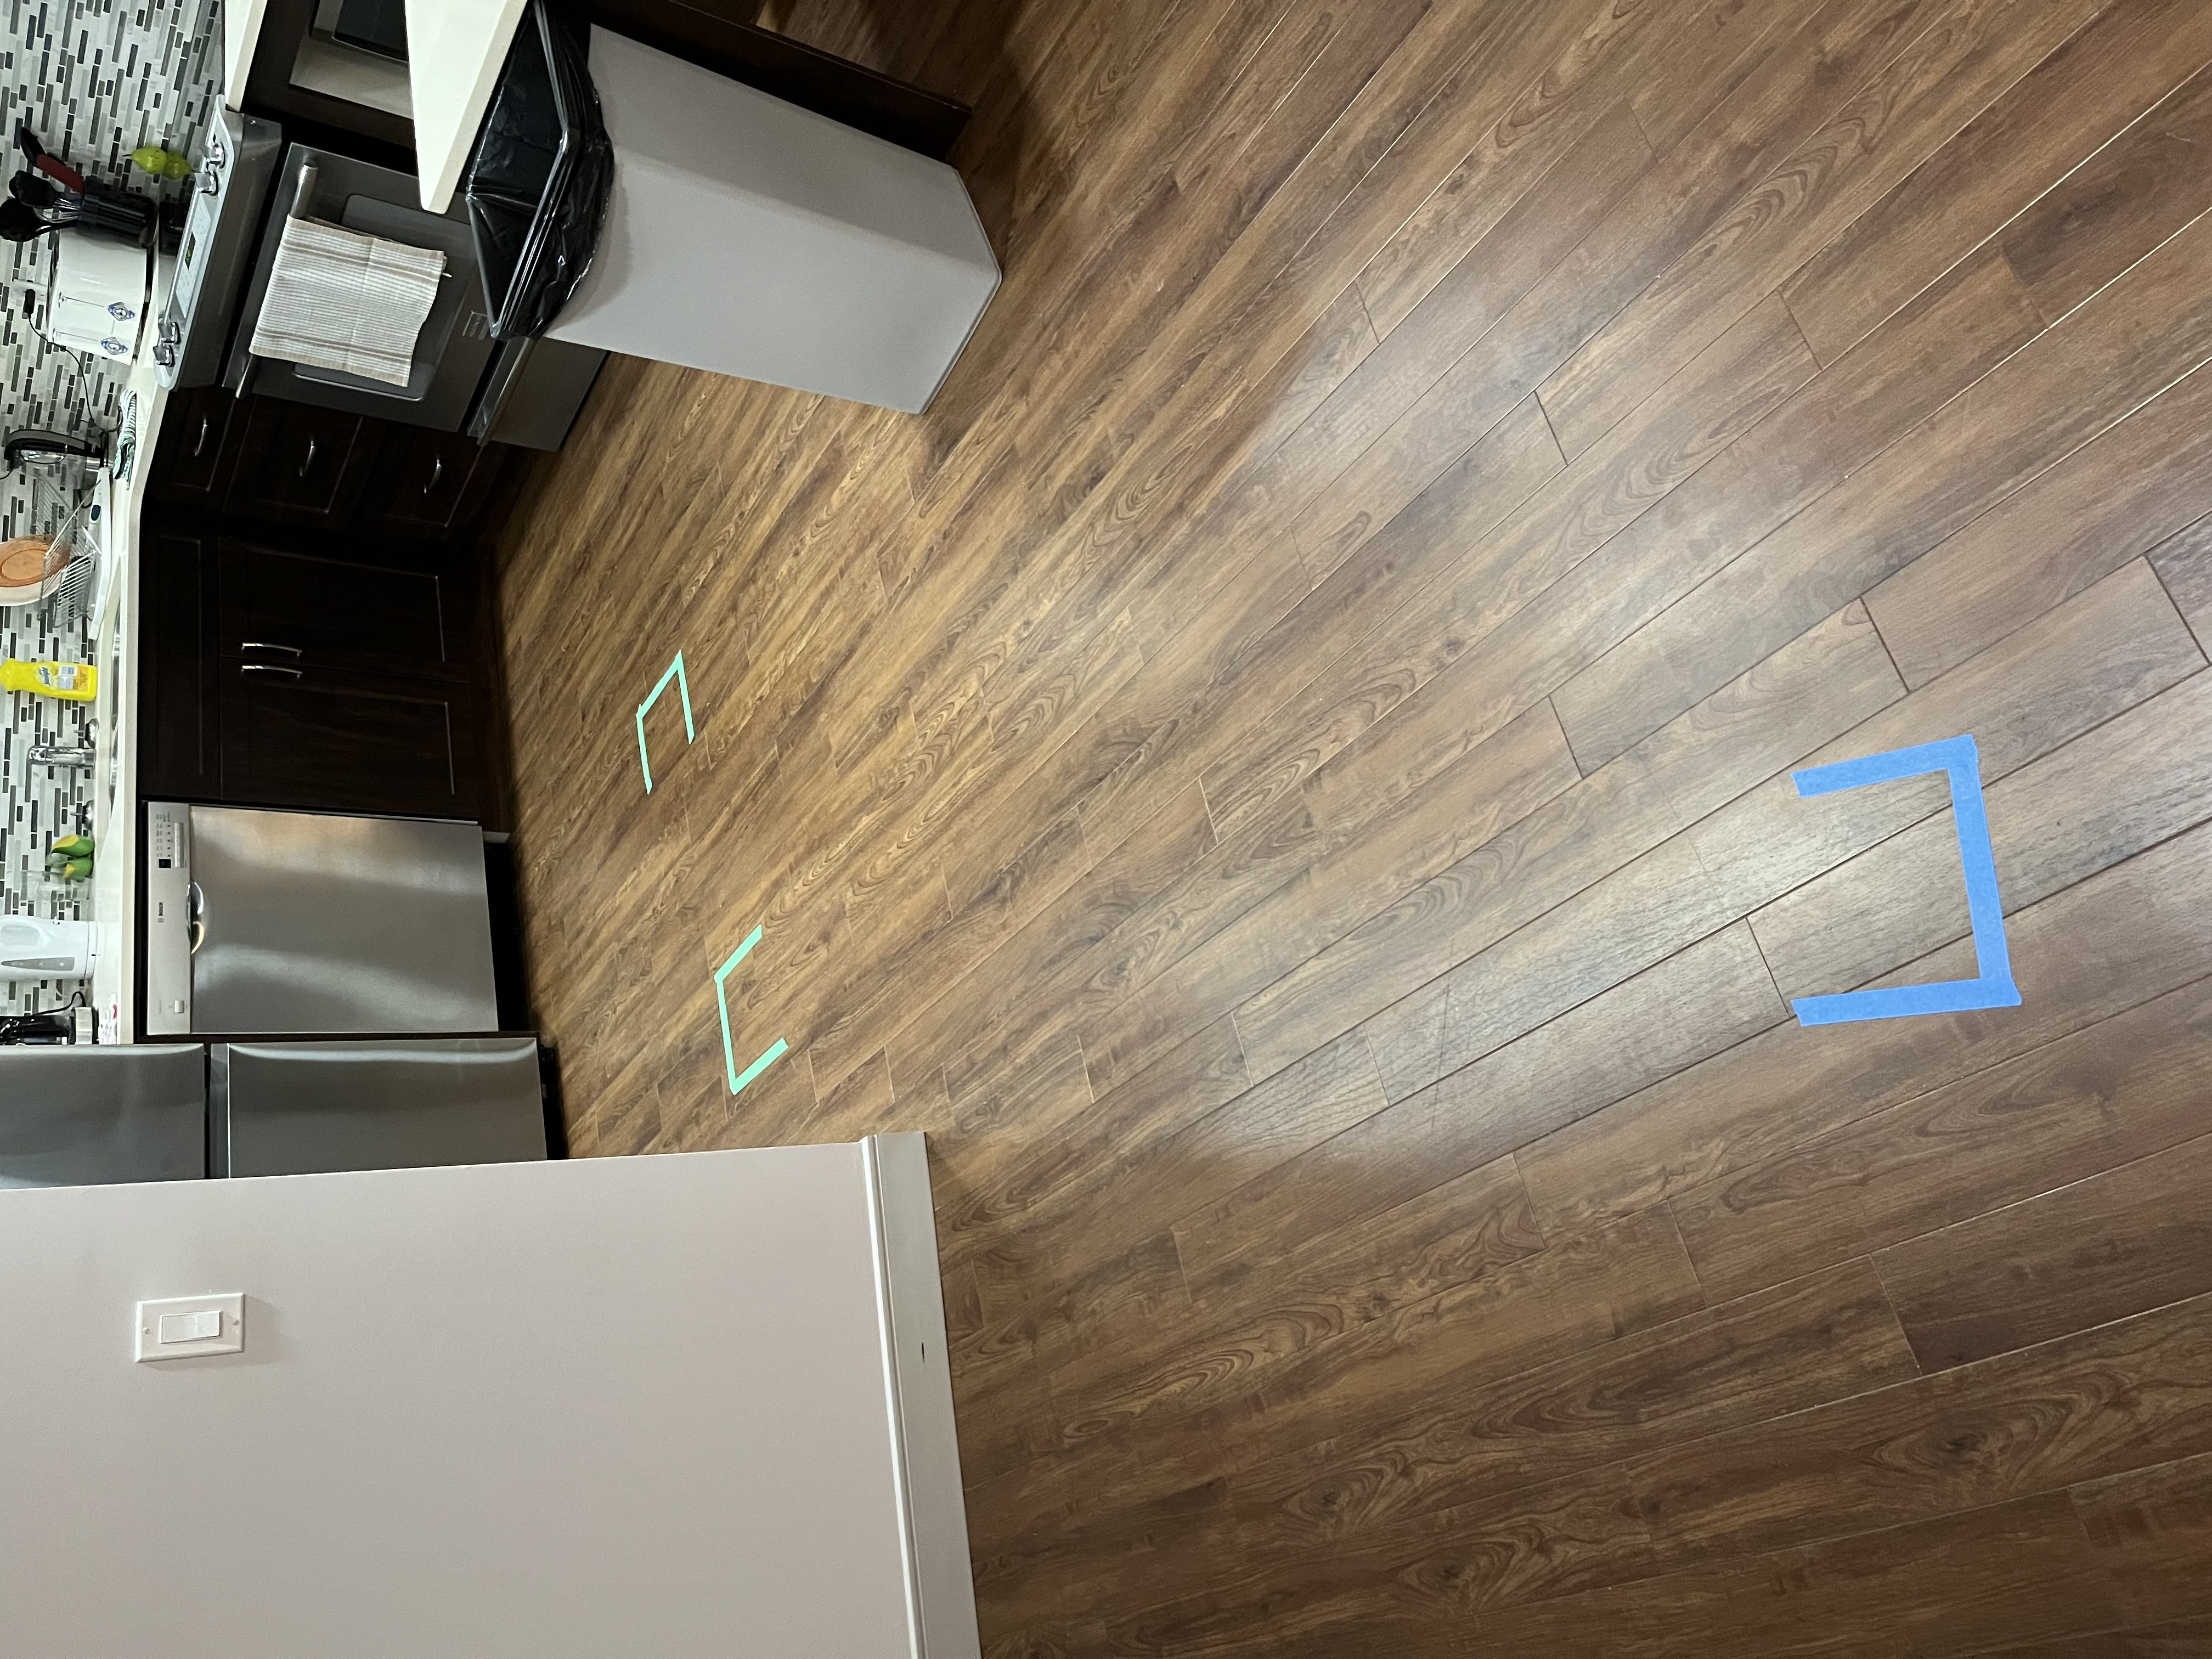
\includegraphics[width=\textwidth, angle=-90]{tape.jpg}
    \caption{Box tape placement at the stove, fridge, and dining table. Participant's toes 
    and sides of feet should touch the tape.}
\end{figure}

Following the tape placement guidelines outlined at the beginning of this section,
tape was placed at or near the following locations. Refer to the AUTOCAD floor plan for 
the location of the rooms (Figure \ref{fig:floorplan}):
\begin{itemize}
    \item The Hallway between Living Room and Kitchen facing the Dining Table.
    \item The Living Room facing the Desk.
    \item The Bedroom facing the bed.
    \item The Hallway between the bedroom and the bathroom, facing away from the wall.
    \item Bathroom facing the toilet.
    \item Kitchen facing the stove.
    \item The Hallway between Living Room and Kitchen facing the Dining Table.
\end{itemize}

\begin{figure}[ht]
    \label{fig:floorplan}
    \centering
    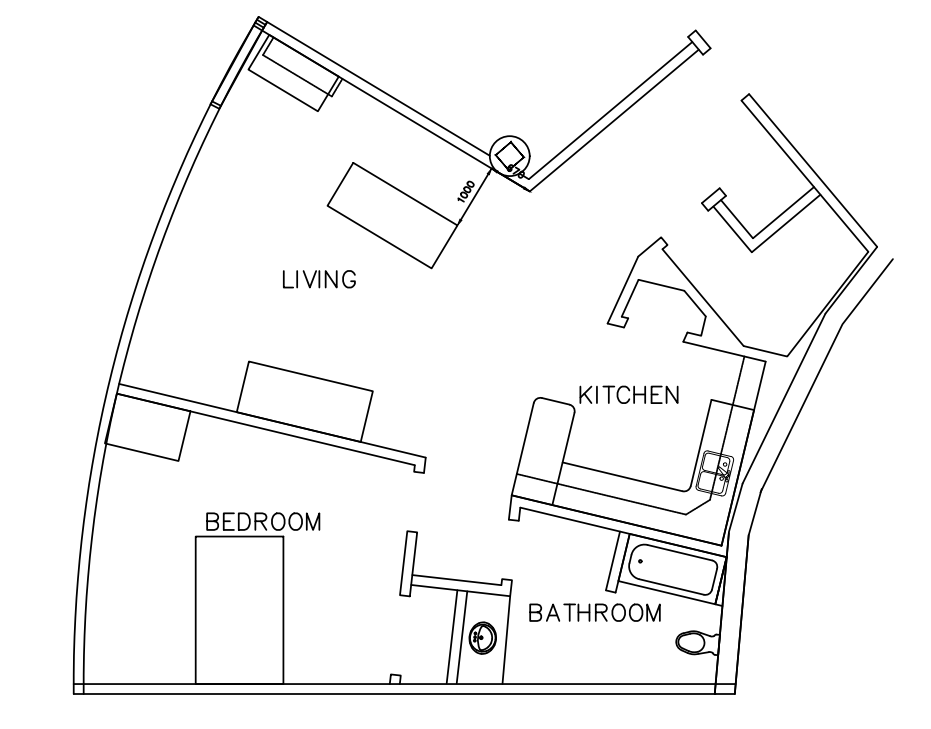
\includegraphics[width=\textwidth]{floorplan}
    \caption{Floor plan of the ILS.}
\end{figure}


\subsection{Protocol}
A stopwatch python script was created with predetermined labels and used as the ground truth 
for positions. A single participant wore the tag on a 3D printed necklace mount (Figure \ref{fig:necklace}). 
The measuring tape was used to measure the height from the ground and height when squatting.
For this participant, the standing height was \textbf{144cm} and the squatting height was \textbf{68.5cm}.

\begin{figure}[ht]
    \label{fig:necklace}
    \centering
    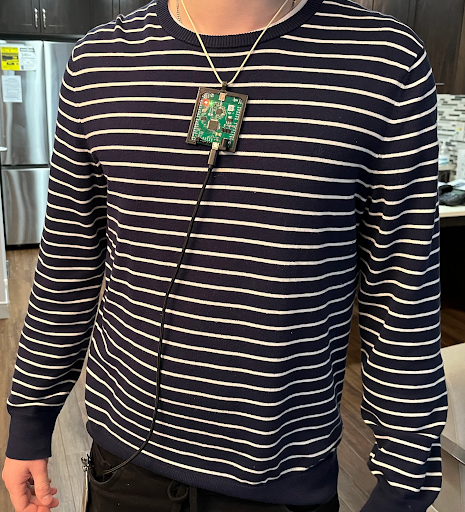
\includegraphics[width=\textwidth]{necklace}
    \caption{The Pozyx tag mounted in a custom 3D printed necklace mount.}
\end{figure}

The protocol had the following steps:
\begin{enumerate}
    \item At the first location (Hallway Between Living Room and Kitchen) stand still for 10 seconds
    \item Squatt still for 10 seconds.
    \item Move to next position.
    \item Repeat steps 1-3 until all of the positions have been reached.
    \item Finally return to the first position (Hallway Between Living Room and Kitchen)
\end{enumerate}

There were 5 trials for each configuration.

\subsection{Analysis}
Trials for each configuration were aggregated, transition periods were removed, 
data of interest was time normalized and the mean and standard deviation of each
location while standing and squatting were recorded.


% ----------------------------------------------------------------------------------------------------
